\section{Übersicht}
\label{section:Übersicht}
Die OpenPEARL Laufzeitumgebung wird um eine Trace-Funktionalität für
\textit{SEMA} Objekte erweitert. Dazu wird die \textit{SEMA} Implementierung in
der OpenPEARL Laufzeitumgebung angepasst. Diese Trace-Funktionalität wird über
eine Umgebungsvariable gesteuert. Das Schreiben auf die Festplatte ist sehr
zeitintensiv, deswegen werden Logeinträge zwischengespeichert und erst bei der
Erreichung eines definierten Werts in die Trace-Datei geschrieben. Dieser Wert
kann ebenfalls über eine Umgebungsvariable definiert werden. 

Die erzeugte Trace-Datei dient als Eingabe für die Anwendung zur Generierung und
Darstellung der chronologischen Verwendung der \textit{SEMA} Objekte.

Zusätzlich wird die Trace-Datei mit Hilfe des MagicLock\footnote{Siehe
\cref{section:MagicLock}} Algorithmus nach potentiellen Deadlocks durchsucht.
Potentielle Deadlocks werden anschließend als gerichteter Graph dargestellt.

\section{Erzeugung der Trace-Datei}
\label{section:Erzeugung der Trace-Datei}
Die Trace-Datei enthält alle benötigten Informationen, um potentielle Deadlocks
zu erkennen:
\begin{enumerate}
  \item Der genaue Zeitpunkt des Ereignisses 
  \item Die Art des Ereignisses (Lock, Unlock)
  \item Die Id des ausführenden Threads
  \item Der Name des betroffenen Lockobjekts
\end{enumerate}

\begin{figure}[ht]
  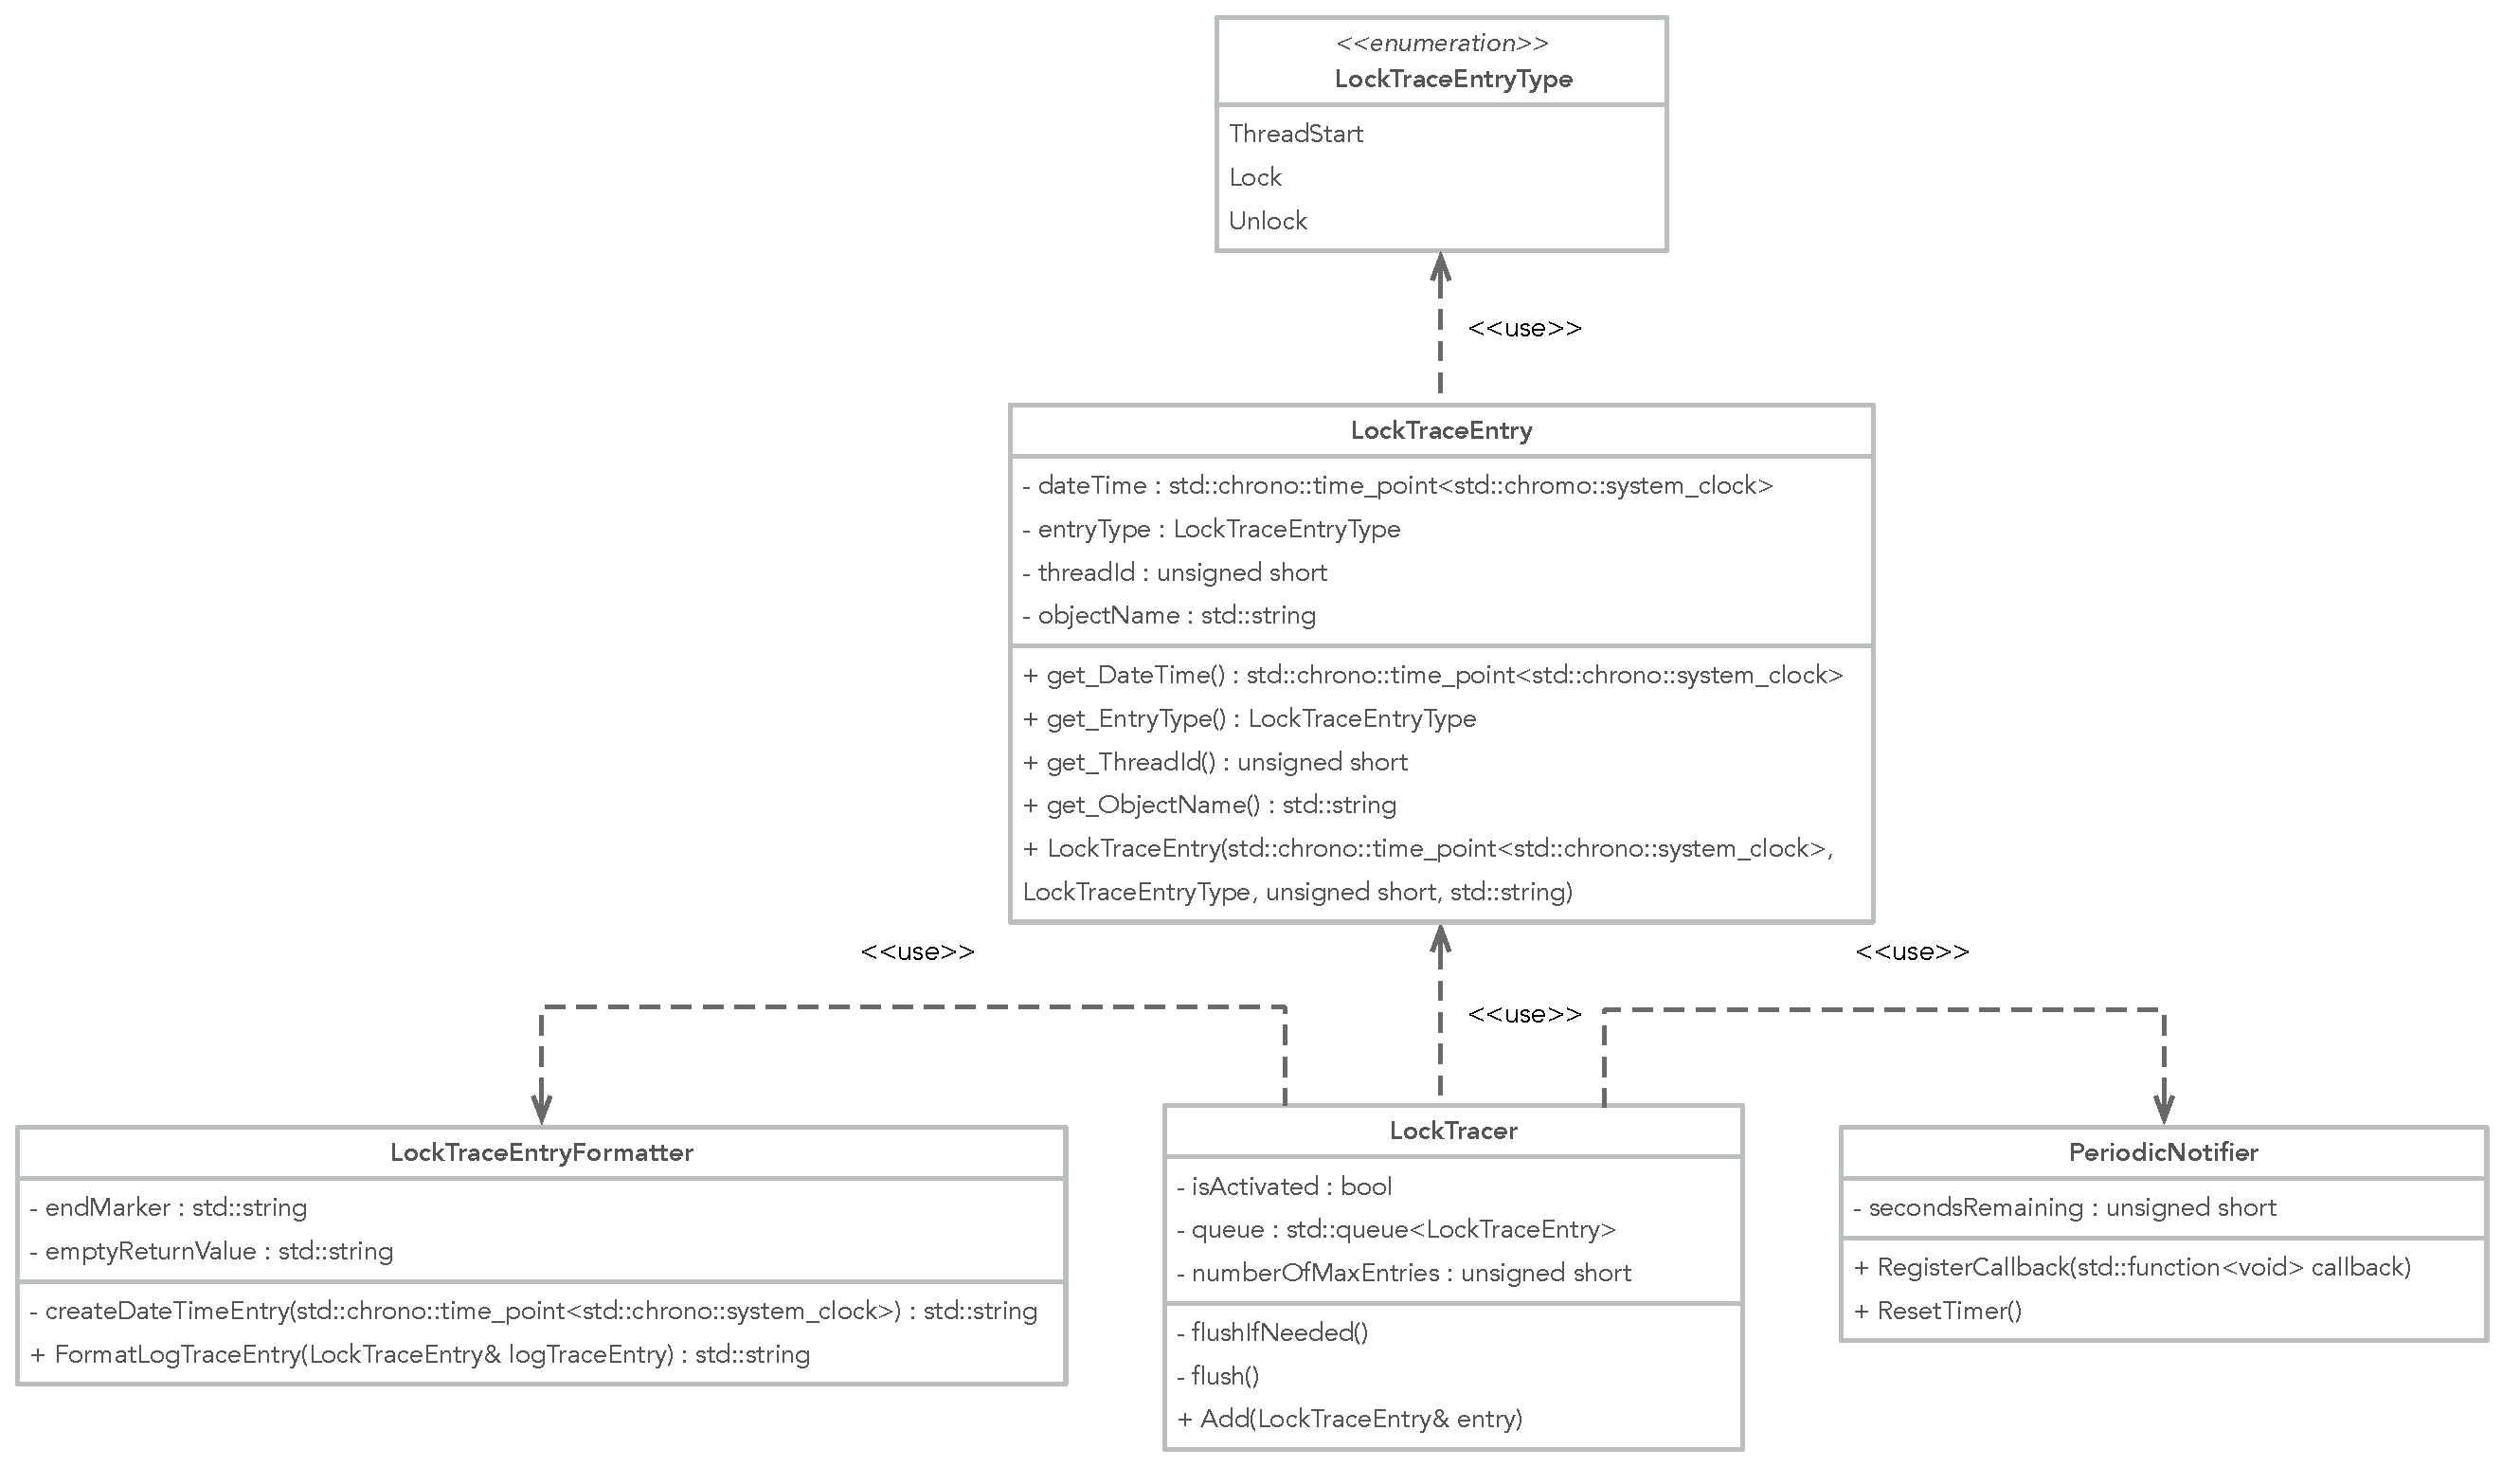
\includegraphics[width=\linewidth]{LockTrace_Design.eps}
  \caption{UML Klassendiagramm für Trace-Funktionalität}
  \label{fig:LockTrace_Design}
\end{figure}

In \cref{fig:LockTrace_Design} sind die benötigten Klassen dargestellt. Die
notwendigen Informationen für einen Trace-Eintrag werden in der Klasse
\texttt{LockTraceEntry} gehalten. Für den Zeitunkt wird der Typ 
\texttt{chrono::time\_point} vom Typ \texttt{chrono::high\_resolution\_clock}
verwendet. Der Typ \texttt{chrono::high\_resolution\_clock} stellt einen
Zeitpunkt mit der höchstmöglichen Genauigkeit der jeweiligen Implementierung dar
{TODO: Referenz auf C++11}. Für die spätere Visualisierung ist eine hohe
Genauigkeit notwendig, um nahezu parallel aufgetretene Lock-Ereignisse
chronologisch getrennt visualisieren zu können. Die Klasse
\texttt{LockTraceEntryFormatter} erstellt mit der Methode
\texttt{FormatLogTraceEntry} aus einem \texttt{LockTraceEntry} eine
Zeichenkette, welche einer Zeile in der Trace-Datei entspricht. Diese Klasse
wird als Singleton implementiert, da zur Laufzeit immer nur genau eine Instanz
benötigt wird. Die Klasse \texttt{LockTracer} stellt die Methode \texttt{Add}
zur Verfügung, welche von der OpenPEARL Laufzeitumgebung aufgerufen wird. Mit
Hilfe der Methode können Lock-Ereignisse erstellt werden. Die Klasse wird
ebenfalls als Singleton implementiert, damit nur eine Instanz zur Laufzeit
verwendet werden kann. Das Speichern der Ereignisse in die Trace-Datei ist
kostspielig und soll daher nicht für jeden Eintrag gemacht werden. Die Klasse
\texttt{LockTracer} reiht dazu die einzelnen Lock-Ereignisse, welche über die
\texttt{Add} Methode hinzugefügt werden, in eine Warteschlange ein. Sobald eine
spezifizierte Anzahl erreicht ist, wird die Warteschlange geleert und in die
Trace-Datei geschrieben. Die Anzahl kann über die Umgebungsvariable
\texttt{OpenPEARL\_LockTracer\_MaxEntries} spezifiziert werden. Die
Umgebungsvariable wird bei der Initialisierung der \texttt{LockTracer}
Implementierung ausgelesen und in der Variable \texttt{numberOfMaxEntries}
gespeichert. Das Hinzufügen der Ereignisse in die Warteschlange kann parallel
erfolgen und muss daher Thread sicher implementiert werden. Eine Möglichkeit
wäre, die einzelnen Zugriffe über einen Lock zu synchronisieren. Dies würde die
Laufzeit der Anwendung stark negativ beeinflussen. Deswegen wird eine lock freie
Implementierung einer Warteschlange verwendet
\autocite{Moody_Camels_Concurrentqueue}. Die Warteschlange garantiert eine
Thread sichere Implementierung, aber keine Sortierung innerhalb der
Warteschlange. Es kann passieren, dass Lock-Ereignisse in einer anderen
Reihenfolge aus der Warteschlange herausgenommen werden als sie eingefügt
wurden. Beim Auslesen der Trace-Datei muss daher anfangs eine Sortierung der
Einträge gemäß ihres Zeitpunkts durchgeführt werden. Der Dateipfad zur
Speicherung der Trace-Datei wird über die Umgebungsvariable
\texttt{OpenPEARL\_LockTracer\_Path} definiert und bei der Initialisierung der
\texttt{LockTracer} Implementierung in der Variable \texttt{filePath}
gespeichert. Die dritte Umgebungsvariable
\texttt{OpenPEARL\_LockTracer\_Enabled} wird zur Aktivierung der
Trace-Funktionalität verwendet. Wenn die Umgebungsvariable gesetzt ist und den
Wert \texttt{true} hat, wird die Trace-Funktionalität aktiviert. Ansonsten
werden alle Aufrufe zur \texttt{Add} Methode direkt über eine \texttt{return}
Anweisung beendet. Dadurch wird die Laufzeit der Anwendung bei deaktivierter
Trace-Funktionalität nicht beeinflusst.

In der OpenPEARL Laufzeitumgebung werden die \textit{REQUEST} und
\textit{RELEASE} Anweisungen in der Semaphore Implementierung unter
runtime/common/Semaphore.cc implementiert. Bei einer Erhöhung oder einer
Verringerung eines Semaphors muss ein Logeintrag erzeugt werden. Bei einer
Erhöhung muss der \texttt{LockTraceEntryType} \texttt{Unlock} bei einer
Verringerung der \texttt{LockTraceEntryType} \texttt{Lock} verwendet werden. Die
Klassen für die Implementierung des LockTracers müssen bei der Kompilierung der
OpenPEARL Laufzeitumgebung mit einbezogen werden. In der Datei
runtime/common/Files.common sind alle Dateien aufgeführt, welche bei der
Kompilierung einbezogen werden. Dort müssen die Dateien, die aus
\cref{fig:LockTrace_Design} entstehen eingetragen werden.

\section{Analysieren der Trace-Datei}
\label{section:Analysieren der Trace-Datei}
Als Eingabe dient die in \cref{section:Erzeugung der Trace-Datei} erzeugte
Trace-Datei. Die chronologische Darstellung wird, wie in
\cref{fig:Timeline_Example} skizziert, über einen zwei dimensionalen Graphen
realisiert. Die Ordinate bildet die Zeit ab, wobei nur das Delta in
Mikrosekunden zwischen den einzelnen Ereignissen dargestellt wird. Für jeden
Thread wird ein Eintrag auf der Abszisse gemacht. Es wird zwischen zwei
Ereignissen unterschieden. Wird ein \texttt{SEMA} Objekt in Besitz genommen,
wird ein roter, für das Freigeben eines \texttt{SEMA} Objekts ein grüner, Kreis
gezeichnet. Die Beschriftung eines Kreises enthält den Namen des \texttt{SEMA}
Objekts.

\begin{figure}[ht]
  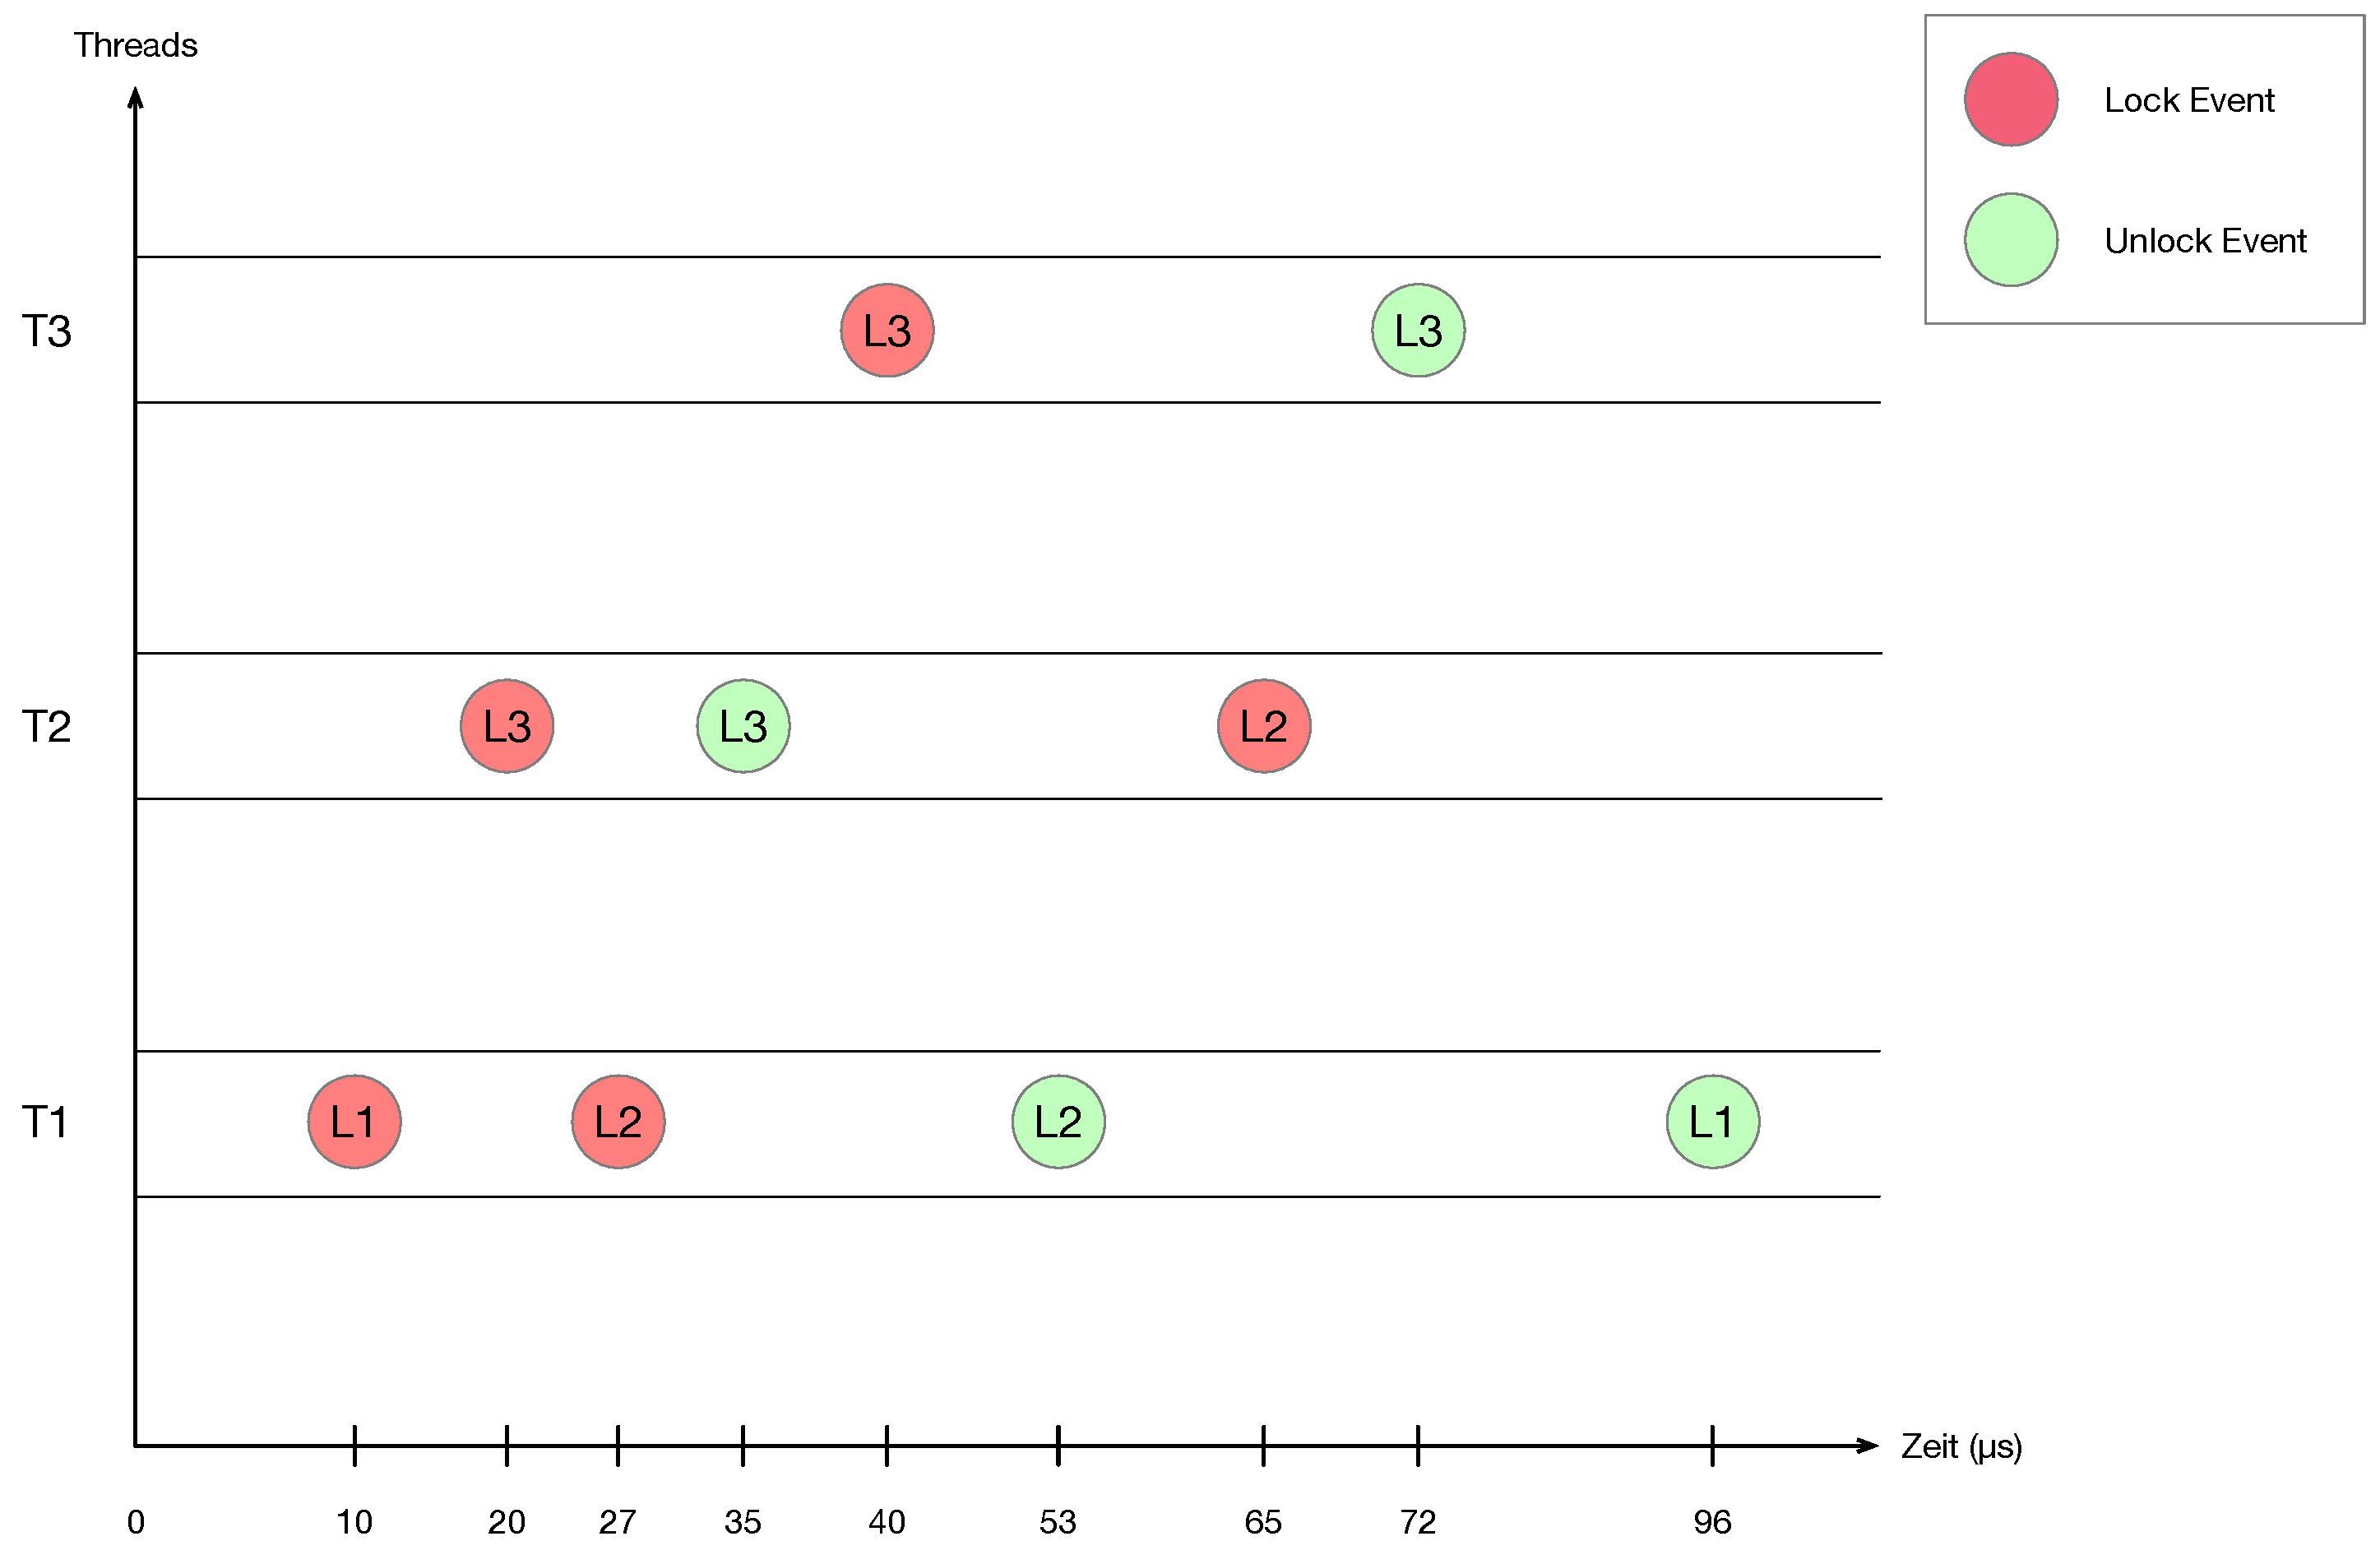
\includegraphics[width=\linewidth]{Timeline_Example.eps}
  \caption{Visualisierung der chronologischen Verwendung von \textit{SEMA} Objekten}
  \label{fig:Timeline_Example}
\end{figure}

\section{Erweiterung: Potenzielle Deadlocks}
\label{section:Erweiterung: Potenzielle Deadlocks}
Der in \cref{section:MagicLock} beschrieben Algorithmus wird dazu verwendet, um
potentielle Deadlocks in der aus \cref{section:Erzeugung der Trace-Datei}
erstellten Trace-Datei zu finden. 

\begin{figure}[ht]
  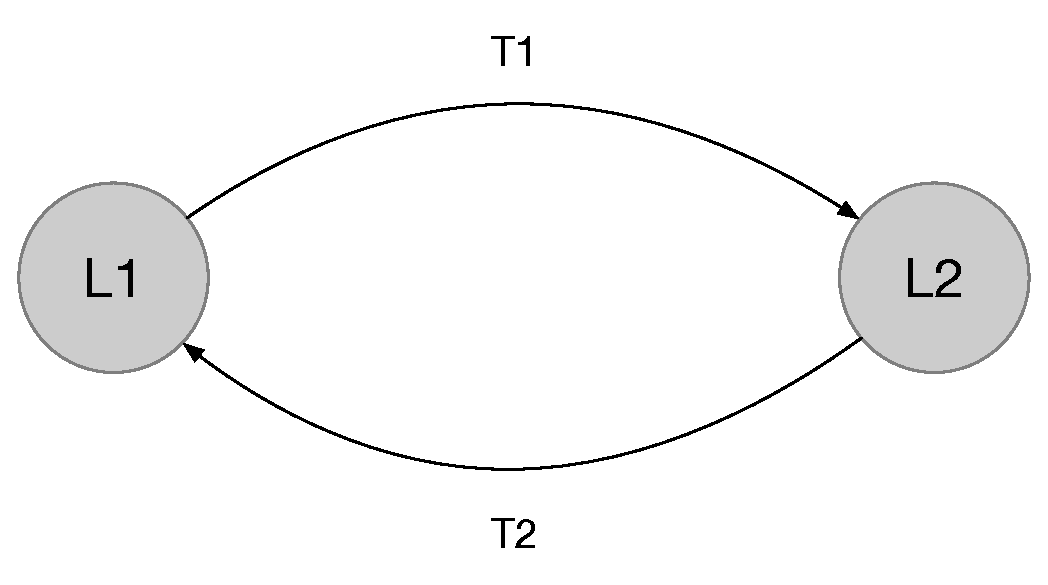
\includegraphics[width=\linewidth/2]{Magiclock_Example.eps}
  \caption{Beispielhafte Visualisierung eines potentiellen Deadlocks}
  \label{fig:Magiclock_Example}
\end{figure}

Potentielle Deadlocks werden wie in \cref{fig:Magiclock_Example} skizziert als
gerichteter Graph dargestellt. Knoten repräsentieren Lockobjekte, Kanten
repräsentieren die Inbesitznahme eines Lockobjekts und die Beschriftung an einer
Kante bezeichnet den ausführenden Thread. In dem skizzierten Beispiel ist ein
potentieller Deadlock zwischen den Threads \textit{T1} und \textit{T2}
dargestellt. Der Thread \textit{T1} nimmt das Lockobjekt \textit{L2} in Besitz
während dieser bereits \textit{L1} besitzt. Dies ist zu erkennen an der Kante
vom Knoten \textit{L1} zum Knoten \textit{L2} mit der Bezeichnung \textit{T1}.
Der Thread \textit{T2} nimmt in dem Beispiel das Lockobjekt \textit{L1} in
Besitz während dieser bereits \textit{L2} besitzt. Dies kann zu einem Deadlock
führen, wenn \textit{T1} das Lockobjekt \textit{L1} und \textit{T2} das
Lockobjekt \textit{L2} gleichzeitig besitzen.